\documentclass[12pt,letterpaper]{article}
\usepackage{fullpage, lastpage, enumerate, fancyhdr, titlesec}
\usepackage[top=2cm, bottom=4.5cm, left=2.5cm, right=2.5cm]{geometry}
\usepackage{amsmath,amsthm,amsfonts,amssymb,amscd}
\usepackage{mathrsfs, xcolor, graphicx, subcaption, siunitx}
\usepackage{hyperref}
\graphicspath{{./images}}

\hypersetup{%
  colorlinks=true,
  linkcolor=blue,
  linkbordercolor={0 0 1}
}

\setlength{\parindent}{0.0in}
\setlength{\parskip}{0.05in}

\titleformat{\subsection}
  {\normalfont\normalsize\itshape}{\thesubsection}{1em}{}

\pagestyle{fancyplain}
\headheight 15pt
\fancyhf[FL]{Matthew Bernstein}
\fancyhf[HR]{\today}
\fancyhf[HL]{ISyE 7406 - Homework 3}
\fancyhf[FC]{}
\fancyhf[FR]{\thepage}
\headsep 1.5em

\title{ISYE 7406 - Homework 3}
\author{Matthew Bernstein}

\begin{document}
\fancypagestyle{plain}{
    \fancyhf{}
    \renewcommand{\headrulewidth}{0pt}
    \renewcommand{\footrulewidth}{0pt}
}
\maketitle
\section*{Introduction}

In this experiment, different methods of fitting and comparing classification models were tested. The dataset included 7 characteristics of cars with fuel efficiency as the response. The goal was to determine a model using the characteristics to determine if a car is expected to have fuel efficiency that is better (or worse) than the median.

Five models were fit after selecting relevant features for 100 Monte Carlo cross validation trials. Accuracy for each model was assessed using classification error of the test set. 

\section*{Exploratory Data Analysis}

The dataset contains 7 characteristics. Of these, 2 are categorical variables: \textit{cylinders} and \textit{origin}. The other 5 are continuous variables. While \textit{year} is listed as a catergorical feature, due to the number of levels and context, it is treated as a continous variable for this analysis. Also, given the low amount of 3 and 5 cylinder vehicles in the dataset, those levels were combined with 4 cylinders. The features are a combination of mechnical information such as \textit{weight} and \textit{acceleration} as well as "biographical" such as \textit{year} and \textit{origin}. 

A pairwise analysis of the categorical variables is show in Figure \ref{fig:cat_vars}. It appears that both variables have correlation with fuel efficiency. Lower cylinder cars are much more likely to have better than median fuel efficiency, as well as cars from region 2 and 3. 

\begin{figure}[!htb]
  \centering
  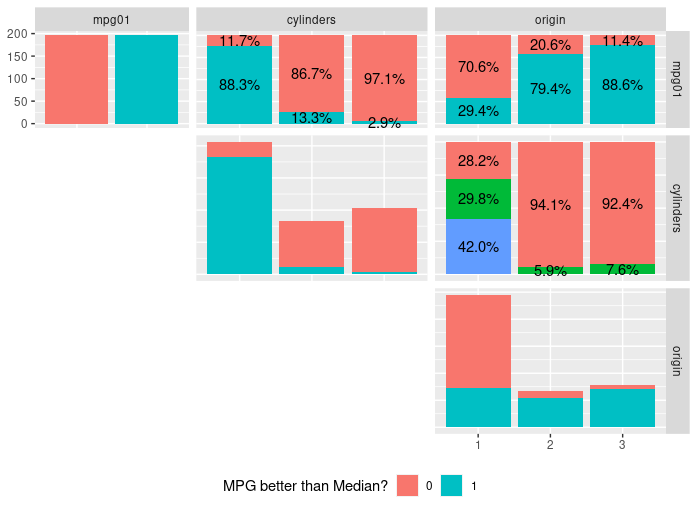
\includegraphics[width=0.6\textwidth]{disc_pairs}
  \caption{Pairwise analysis of categorical variables}
  \label{fig:cat_vars}
\end{figure}

Figure \ref{fig:cont_vars} shows a pairwise analysis of the continuous variables while Figure \ref{fig:cor} shows the correlation heatmap. \textit{Displacement}, \textit{weight}, and \textit{horsepower} all are very strong predictors of fuel efficiency. The correlation heatmap shows extremely high colinearity between those variables as well. It is likely that only one of those variables is required for a strong classifier. \textit{Year} appears to show a weak correlation to fuel efficiency with later years having better odds of being above the median. \textit{Acceleration} appears to be the least correlated and might not be needed for a classifier.

\begin{figure}[!htb]
  \centering
  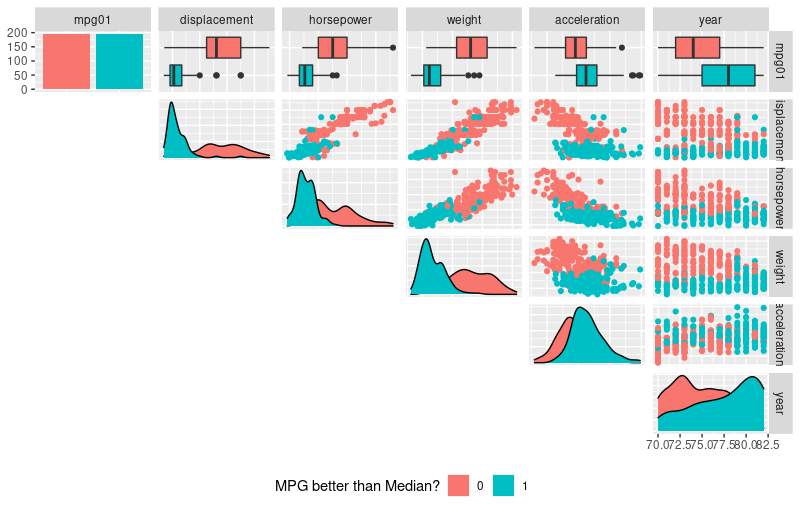
\includegraphics[width=0.6\textwidth]{cont_pairs}
  \caption{Pairwise analysis of continuous variables}
  \label{fig:cont_vars}
\end{figure}

\begin{figure}[!htb]
  \centering
  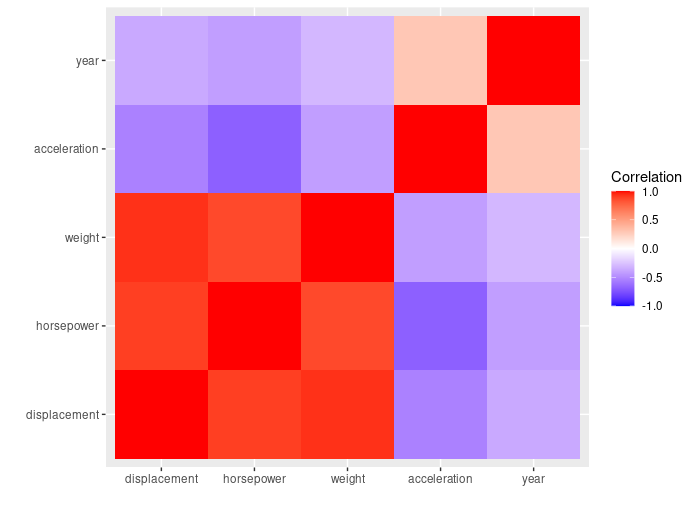
\includegraphics[width=0.6\textwidth]{heatmap}
  \caption{Correlation heatmap}
  \label{fig:cor}
\end{figure}

\section*{Methodology}

\subsection*{Variable Selection}
In order to simplify the model, two rounds of variable selection were performed.

\subsubsection*{Acceleration}
Of all the continuous variables, \textit{acceleration} seems the least likely to impact the gas milage. Two logisitic regression models were made, one with all variables and one with all variables except for \textit{aceeleration}. Each model was trained on all data with 5-fold cross validation, repeated 3 times. The cross validation accuracy and AIC are shown in Table \ref{tab:accel_varsel}. 

\begin{table}[hbt!]
  \caption{\label{tab:accel_varsel}Acceleration variable selection results}
  \centering
  \begin{tabular}{|l|r|r|}
  \hline
  Model & Accuracy & AIC\\
  \hline
  Full & 0.9090 & 159.4781\\
  \hline
  Without Acceleration & 0.9115 & 157.8898\\
  \hline
  \end{tabular}
\end{table}

Moving forward, \textit{acceleration} was omitted from the feature set.

\subsubsection*{Displacement, Weight, Horsepower}
There was high colinearity between \textit{displacement}, \textit{weight}, \textit{horsepower}. It is likely that only one of those three variables is sufficient for the model. Four models were created, one with all variables and one model each excluding two of the three variables in this round of selection. Each model was trained on all data with 5-fold cross validataion, repeated 3 times. The cross validation accuracy and AIC are shown in Table \ref{tab:dwh_varsel}

\begin{table}[hbt!]
  \caption{\label{tab:dwh_varsel}Displacement, weight, horsepower variable selection results}
  \centering
  \begin{tabular}{|l|r|r|}
  \hline
  Model & Accuracy & AIC\\
  \hline
  Full & 0.9064 & 157.8898\\
  \hline
  Only Displacement & 0.9098 & 195.0084\\
  \hline
  Only Weight & 0.9183 & 162.3589\\
  \hline
  Only HP & 0.8928 & 187.9729\\
  \hline
  \end{tabular}
 \end{table}

All future models were created with \textit{displacement} and \textit{horsepower} omitted.

\subsection*{Model Comparisons}

Five models were created for comparison: Logistic Regression, Linear Discriminant Analysis (LDA), Quadratic Discriminant Analysis (QDA), Naive Bayes Classifier, and K-Nearest Neighbors classifier. For the KNN model, $k$ was chosen using a 3 times repeated, 5-fold cross validation. All models were subject to 100 trials of Monte Carlo cross validation. For the KNN model, the optimal $k$ was determined each trial. 

The test error was reported for each trial and aggregated. 

\section*{Results}

After 100 Monte Carlo cross validation trials, the aggregated test errors are shows in Table \ref{tab:results}.

\begin{table}[hbt!]
  \caption{\label{tab:results}Aggregated model test classification error}
  \centering
  \begin{tabular}{|l|r|r|r|}
  \hline
    & Mean & Median & Variance\\
  \hline
  Logistic Regression & 0.9158 & 0.9103 & 0.0008\\
  \hline
  Naive Bayes & 0.9040 & 0.9103 & 0.0008\\
  \hline
  LDA & 0.9035 & 0.9103 & 0.0008\\
  \hline
  QDA & 0.8981 & 0.8974 & 0.0008\\
  \hline
  KNN & 0.8719 & 0.8718 & 0.0011\\
  \hline
  \end{tabular}
\end{table}

As expected, the Logistic Regression model performed the strongest. Logisitic Regression is the most robust of the model choices since it makes no assumptions about the data. Naive Bayes and LDA performed similarly. Although, they also make assumptions on the data, it appears the common covariance assumption that LDA assigns is more accurate than the per-class normality assumption that QDA makes. Given that the model variables were downsized and sources of colinearity were removed, it follows that the independence assumption that Naive Bayes classifiers make would be more accurate. However, I suspect that removing those variables hurt the accuracy of the KNN classifier since those variables would help close distance between applicable neighbors. It is also possible that transforming the continuous response to a discrete variable could cause misclassification on points near the boundary.

\section*{Conclusion}

When creating a classification model, there are many options to evaluate. LDA, QDA, and Naive Bayes place assumptions upon the dataset which can cause them to fall in prediction accuracy. KNN models are also an option however they are susceptible to data quality issues and unimportant features. Logisitic regressions are usually the most robust models and the analysis on this dataset supports this. In conclusion, I would recommend using logisitic regression models for classification. 

\end{document}